\section{Compression attacks}\label{sec:attack}

\subsection{A high-level overview}\label{subsec:example}
Compression side-channel attacks pose a serious threat
against TLS and any encryption system in general.
Although widely acknowledged and documented by the security community, there
still exist too few mitigation strategies to thwart them, primarily due to
(i) the perceived high performance penalty associated with mitigating them, and
(ii) the perceived complexity that results in a lack of production code tools to allow for
the robust execution of such attacks. In this work we illustrate that these
perceptions are wrong and the continuous existence of such realistic threats
suggests a grave situation that needs to be addressed.

In order to appreciate the seriousness of these attacks we begin a high-level
overview.

Suppose that a user browses the Internet and accesses a website, e.g. a social
network or a service that handles sensitive private data. When she requests a
page on this site, the server collects all needed data, generates the HTML code
age and sends a response over the network containing the page's code.  All response
data is encrypted under TLS, which ensures privacy and integrity for this
communication, and compressed for efficiency.

Consider now an adversary who aims to break this communication's security by
effectively revealing information about the exchanged private data. He decides
to mount a compression side-channel attack, so he must first make sure that
certain conditions are met.

Firstly, the adversary has a passive level of network access. That way he is
able to collect and analyze the network packets of the encrypted communication
with the server.

Secondly, he is able to issue any number of malicious requests using the user's
cookies (which will be encrypted). He can achieve this by forcing the user's
browser to run a piece of code, such as a Javascript script. This script will be
either hosted on an adversary-controlled website or injected in plain HTTP
responses from third websites, in which case the adversary also needs active
level of network access. When loaded in the user's browser, the script
can issue requests to any URL crafted by the adversary. Figure
\ref{fig:attack_model} elaborates on this attack mode.

Thirdly, the website under attack allows data injection in the encrypted
plaintext. This data takes the form of a specially crafted ``reflection'' string
that the adversary includes in the malicious requests. Depending on where the
targeted secret exists, the reflection need be included in either the
request, as is the case of CRIME which targets authentication cookies, or the
response plaintext, like the case of BREACH targeting CSRF tokens
\cite{de2011automatic}.

The adversary issues the attack in stages. In each stage he creates a pool of
reflections and makes malicious requests for each reflection in the pool.  As
the attack progresses the adversary collects network data related to multiple
requests and reflections.  Although this data is encrypted, analysis on the
packet lengths can reveal otherwise hidden properties of the private data.  An
attack stage ends when the adversary has successfully decrypted a single
character in the secret. We will elaborate on the form of the reflections and
the analysis in section \ref{subsec:rupture}.

At this point the privacy of the communication between the user and the website
has been compromised, since the adversary has broken the confidentiality of the messages
by effectively circumventing TLS security.

    \begin{figure}[thpb]
        \centering
            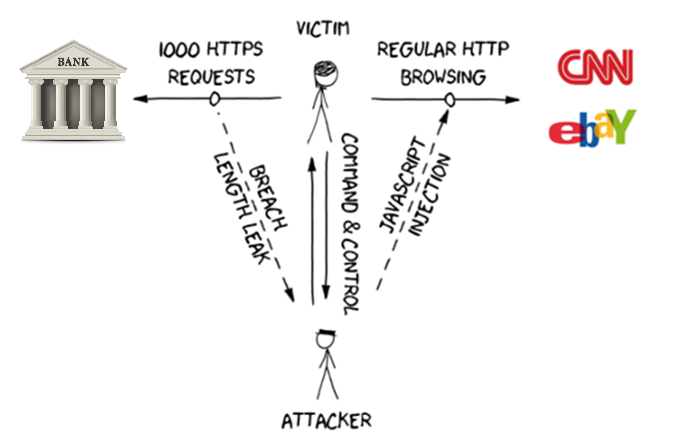
\includegraphics[width=0.48\textwidth]{figures/attack_model.png}
        \caption{The attack model}
        \label{fig:attack_model}
    \end{figure}

\subsection{A motivating example, concepts and notations}\label{subsec:terms}
We now describe a concrete example of the scenario in the previous section to
illustrate the various terms we use in the rest of this paper.

The target of the attack is a mail service found in the URL
\textit{mail.example.com}. The victim is a user that is logged in this service
and browses the Internet.

The web page that the adversary exploits is
\textit{\url{mail.example.com/search?query=attack}}. This page provides the HTTP
GET parameter \textit{query} and an example of a reflection that the adversary
uses is the string \textit{attack}. The HTML response for this request is:

\begin{lstlisting}[basicstyle=\small\ttfamily]
<div>
    <p>You searched for: attack</p>
    <p>No results found.</p>
</div>
<div>
    Your inbox:
    <ul>
    <li>[Bank] Routing number: 123</li>
    </ul>
</div>
\end{lstlisting}

Using the terms introduced in the following sections, the server's function
that generates the HTML code
is an instance of the \textit{rendering function} $f$. The output of $f$ is the
\textit{rendered message} $m$, in our example the HTML response.

The response contains multiple data elements. A data element can be a
\textit{secret}, \textit{static}, or a \textit{reflection}.

A \textit{secret} $s$ is any part of the response that the application wishes to
keep private. Examples of secrets include private messages, financial data, and
web security elements like CSRF tokens. In our example,
the strings ``Bank", which is an email topic, and ``Routing number: 123", which
is the email body, are both secrets.

\textit{Static} is any content that remains unchanged across requests.  Examples
of static data is HTML code, like ``div", or strings like ``Your inbox:" in our
example.  Static content is predictable and thus irrelevant to the attack.

A \textit{reflection} $r$ is a component crafted by the attacker that can be
adaptively transformed as the attack progresses. In this case, the HTTP GET
value ``attack" is a reflection. This string is included in the response in ``You
searched for: attack", an information message for the user used in every
search request.

Secrets are chosen from the distribution $\mathcal{M}$, which in this case
contains all routing numbers and 4-letter strings like ``Bank".

The compression function $\textrm{Com}$ is the compression algorithm used on the
HTML response plaintext. In our example, this algorithm is DEFLATE, the most
common compression algorithm on the web.

The encryption function $\textrm{Enc}$ is the encryption algorithm used by the
web server, the most common today being AES \cite{daemen2013design}. We use the function
$\mathcal{E}$ to describe the composition of $\textrm{Enc}$ and $\textrm{Com}$.

The input of $\mathcal{E}$ is the message $m$ and its output is the
ciphertext $c$ that is sent in the response packets and is sniffed by the
adversary over-the-wire.
